% Chapter 0: Seminar - Time Series Fundamentals
% Harvard-quality academic presentation
% Bachelor program, Bucharest University of Economic Studies

\documentclass[9pt, aspectratio=169, t]{beamer}

% Ensure content fits on slides
\setbeamersize{text margin left=8mm, text margin right=8mm}

%=============================================================================
% THEME AND STYLE CONFIGURATION
%=============================================================================
\usetheme{default}
% Using default theme for clean header/footer control

% Color Palette (matching Redispatch PDF)
\definecolor{MainBlue}{RGB}{26, 58, 110}
\definecolor{AccentBlue}{RGB}{26, 58, 110}
\definecolor{IDAred}{RGB}{205, 0, 0}
\definecolor{DarkGray}{RGB}{51, 51, 51}
\definecolor{MediumGray}{RGB}{128, 128, 128}
\definecolor{LightGray}{RGB}{248, 248, 248}
\definecolor{VeryLightGray}{RGB}{235, 235, 235}
\definecolor{KeynoteGray}{RGB}{218, 218, 218}
\definecolor{SectionGray}{RGB}{120, 120, 120}
\definecolor{FooterGray}{RGB}{100, 100, 100}
\definecolor{Crimson}{RGB}{220, 53, 69}
\definecolor{Forest}{RGB}{46, 125, 50}
\definecolor{Amber}{RGB}{181, 133, 63}
\definecolor{Orange}{RGB}{230, 126, 34}
\definecolor{Purple}{RGB}{142, 68, 173}

% Gradient background (exact Keynote 315° gradient: white to RGB 218,218,218)
\setbeamertemplate{background}{%
    \begin{tikzpicture}[remember picture, overlay]
        \shade[shading=axis, shading angle=315,
        top color=white, bottom color=KeynoteGray]
        (current page.south west) rectangle (current page.north east);
    \end{tikzpicture}%
}
% Fallback solid color for compatibility
\setbeamercolor{background canvas}{bg=}

\setbeamercolor{palette primary}{bg=MainBlue, fg=white}
\setbeamercolor{palette secondary}{bg=MainBlue!85, fg=white}
\setbeamercolor{palette tertiary}{bg=MainBlue!70, fg=white}
\setbeamercolor{structure}{fg=MainBlue}
\setbeamercolor{title}{fg=IDAred}
\setbeamercolor{frametitle}{fg=IDAred, bg=}
\setbeamercolor{block title}{bg=MainBlue, fg=white}
\setbeamercolor{block body}{bg=VeryLightGray, fg=DarkGray}
\setbeamercolor{block title alerted}{bg=Crimson, fg=white}
\setbeamercolor{block body alerted}{bg=Crimson!8, fg=DarkGray}
\setbeamercolor{block title example}{bg=Forest, fg=white}
\setbeamercolor{block body example}{bg=Forest!8, fg=DarkGray}
\setbeamercolor{item}{fg=MainBlue}

% Footer colors (override Madrid theme blue)
\setbeamercolor{author in head/foot}{fg=FooterGray, bg=}
\setbeamercolor{title in head/foot}{fg=FooterGray, bg=}
\setbeamercolor{date in head/foot}{fg=FooterGray, bg=}
\setbeamercolor{section in head/foot}{fg=FooterGray, bg=}
\setbeamercolor{subsection in head/foot}{fg=FooterGray, bg=}

% Bullet styles (apply everywhere including blocks)
\setbeamertemplate{itemize item}{\color{MainBlue}$\boxdot$}
\setbeamertemplate{itemize subitem}{\color{MainBlue}$\blacktriangleright$}
\setbeamertemplate{itemize subsubitem}{\color{MainBlue}\tiny$\bullet$}
\setbeamertemplate{itemize/enumerate body begin}{\normalsize}
\setbeamertemplate{itemize/enumerate subbody begin}{\normalsize}

% Item spacing - compact style
\setlength{\leftmargini}{10pt}       % Level 1: minimal indent
\setlength{\leftmarginii}{10pt}      % Level 2: minimal additional indent
% Compact list spacing (zero extra space before/after lists in blocks)
\makeatletter
\def\@listi{\leftmargin\leftmargini \topsep 0pt \parsep 0pt \itemsep 0pt}
\def\@listii{\leftmargin\leftmarginii \topsep 0pt \parsep 0pt \itemsep 0pt}
\makeatother

\setbeamertemplate{navigation symbols}{}

%=============================================================================
% CUSTOM HEADLINE
%=============================================================================
\setbeamertemplate{headline}{%
    \vskip10pt%
    \hbox to \paperwidth{%
        \hskip0.5cm%
        {\small\color{FooterGray}\renewcommand{\hyperlink}[2]{##2}\insertsectionhead}%
        \hfill%
        \textcolor{FooterGray}{\small\insertframenumber}%
        \hskip0.5cm%
    }%
    \vskip4pt%
    {\color{FooterGray}\hrule height 0.4pt}%
}

%=============================================================================
% CUSTOM FOOTER
%=============================================================================
\usepackage{fontawesome5}

\setbeamertemplate{footline}{%
    {\color{FooterGray}\hrule height 0.4pt}%
    \vskip4pt%
    \hbox to \paperwidth{%
        \hskip0.5cm%
        \textcolor{FooterGray}{\small Time Series Analysis and Forecasting}%
        \hfill%
        \raisebox{-0.1em}{%
            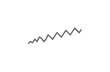
\begin{tikzpicture}[x=0.08em, y=0.08em, line width=0.4pt]
                \draw[FooterGray] (0,3) -- (1,4) -- (2,3.5) -- (3,5) -- (4,4) -- (5,6) -- (6,5.5) -- (7,4) -- (8,5) -- (9,7) -- (10,6) -- (11,5) -- (12,6.5) -- (13,8) -- (14,7) -- (15,6) -- (16,7.5) -- (17,9) -- (18,8) -- (19,7) -- (20,8.5) -- (21,10) -- (22,9) -- (23,8) -- (24,9.5);
            \end{tikzpicture}%
        }%
        \hskip0.5cm%
    }%
    \vskip6pt%
}

%=============================================================================
% PACKAGES
%=============================================================================
\usepackage[utf8]{inputenc}
\usepackage[T1]{fontenc}
\usepackage[english]{babel}
\usepackage{amsmath, amssymb, amsthm}
\usepackage{mathtools}
\usepackage{bm}
\usepackage{tikz}
\usetikzlibrary{arrows.meta, positioning, shapes, calc, decorations.pathreplacing, shadings}
\usepackage{booktabs}
\usepackage{multirow}
\usepackage{array}
\usepackage{graphicx}
\usepackage{hyperref}
\usepackage{colortbl}
\hypersetup{colorlinks=true, linkcolor=MainBlue, urlcolor=MainBlue}
\graphicspath{{../../logos/}{../../charts/}}
\hfuzz=2pt  % Suppress tiny overfull warnings (<2pt)
\vfuzz=2pt  % Suppress tiny vertical overfull warnings (<2pt)

%=============================================================================
% QUANTLET COMMAND
%=============================================================================
\newcommand{\quantlet}[2]{%
    \hfill\href{#2}{%
        \raisebox{-0.15em}{\includegraphics[height=0.7em]{ql_logo.png}}%
        \textcolor{MainBlue}{\tiny\ #1}%
    }%
}

%=============================================================================
% CUSTOM COMMANDS
%=============================================================================
\newcommand{\E}{\mathbb{E}}
\newcommand{\Var}{\text{Var}}
\newcommand{\Cov}{\text{Cov}}
\newcommand{\Corr}{\text{Corr}}
\newcommand{\R}{\mathbb{R}}
\newcommand{\RMSE}{\text{RMSE}}
\newcommand{\MAE}{\text{MAE}}
\newcommand{\MAPE}{\text{MAPE}}

\newcommand{\correct}{\textcolor{Forest}{\checkmark}}
\newcommand{\incorrect}{\textcolor{Crimson}{\texttimes}}

%=============================================================================
% CUSTOM TITLE PAGE
%=============================================================================
\defbeamertemplate*{title page}{hybrid}[1][]
{
    \vspace{0.2cm}
    % Logos row - top header (with clickable links)
    \begin{center}
        \href{https://www.ase.ro}{\includegraphics[height=1.0cm]{ase_logo.png}}\hspace{0.3cm}%
        \href{https://theida.net}{\includegraphics[height=1.0cm]{ida_logo.png}}\hspace{0.3cm}%
        \href{https://blockchain-research-center.com}{\includegraphics[height=1.0cm]{brc_logo.png}}\hspace{0.3cm}%
        \href{https://www.ai4efin.ase.ro}{\includegraphics[height=1.0cm]{ai4efin_logo.png}}\hspace{0.3cm}%
        \href{https://ipe.ro/new}{\includegraphics[height=1.0cm]{acad_logo.png}}\hspace{0.3cm}%
        \href{https://www.digital-finance-msca.com}{\includegraphics[height=1.0cm]{msca_logo.png}}%
    \end{center}

    \vspace{0.6cm}

    % Main title with Q logos on sides (with clickable links)
    \begin{center}
        \begin{minipage}{0.1\textwidth}
            \centering
            \href{https://quantlet.com}{\includegraphics[height=1.1cm]{ql_logo.png}}
        \end{minipage}%
        \begin{minipage}{0.78\textwidth}
            \centering
            {\LARGE\bfseries\usebeamercolor[fg]{title}\inserttitle}

            \vspace{0.3cm}

            {\usebeamerfont{subtitle}\usebeamercolor[fg]{title}\insertsubtitle}
        \end{minipage}%
        \begin{minipage}{0.1\textwidth}
            \centering
            \href{https://quantinar.com}{\includegraphics[height=1.1cm]{qr_logo.png}}
        \end{minipage}
    \end{center}

    \vspace{0.6cm}

    % Authors (left aligned)
    \hspace{0.5cm}{\usebeamerfont{author}\insertauthor}

    \vspace{0.3cm}

    % Institute/Affiliations (left aligned)
    \hspace{0.5cm}\begin{minipage}[t]{0.9\textwidth}
        \raggedright\small\insertinstitute
    \end{minipage}
}

%=============================================================================
% TITLE INFORMATION
%=============================================================================
\title[Time Series Analysis]{Time Series Analysis and Forecasting}
\subtitle{Seminar 0: Fundamentals}
\author[D.T. Pele]{Daniel Traian PELE}
\institute{Academia de Studii Economice din Bucure\c{s}ti\\
IDA Institute Digital Assets\\
Blockchain Research Center\\
AI4EFin Artificial Intelligence for Energy Finance\\
Academia Rom\^{a}n\u{a}, Institutul de Prognoz\u{a} Economic\u{a}\\
MSCA Digital Finance}
\date{}

\begin{document}

% Title page (no header/footer)
{
\setbeamertemplate{headline}{}
\setbeamertemplate{footline}{}
\begin{frame}
    \titlepage
\end{frame}
}

%=============================================================================
% TABLE OF CONTENTS
%=============================================================================
\begin{frame}{Seminar Structure}
    \textbf{\large Seminar structure:}

    \vspace{0.4cm}

    \begin{enumerate}
        \item[\textcolor{MainBlue}{\textbf{1.}}] \textbf{Multiple Choice Quiz} -- Knowledge check
        \vspace{0.15cm}
        \item[\textcolor{MainBlue}{\textbf{2.}}] \textbf{True/False} -- Conceptual checks
        \vspace{0.15cm}
        \item[\textcolor{MainBlue}{\textbf{3.}}] \textbf{Calculation Exercises} -- Applied practice
        \vspace{0.15cm}
        \item[\textcolor{MainBlue}{\textbf{4.}}] \textbf{AI-Assisted Exercises} -- Human vs.\ AI analysis
        \vspace{0.15cm}
        \item[\textcolor{MainBlue}{\textbf{5.}}] \textbf{Summary} -- Key takeaways
    \end{enumerate}
\end{frame}

%=============================================================================
% MULTIPLE CHOICE QUIZ
%=============================================================================
\section{Multiple Choice Quiz}

\begin{frame}{Quiz 1: Time Series Basics}
    \begin{alertblock}{Question}
        Which of the following is NOT a characteristic of time series data?
    \end{alertblock}

    \vspace{0.4cm}
    \begin{enumerate}[A.]
        \item Observations are ordered in time
        \item Consecutive observations are usually correlated
        \item Observations are independent and identically distributed
        \item Data has a natural temporal ordering
    \end{enumerate}

    \vspace{0.5cm}

    \begin{center}
        \textit{Answer on next slide...}
    \end{center}
\end{frame}

\begin{frame}{Quiz 1: Answer}
    \begin{exampleblock}{Answer: C -- Observations are independent and identically distributed}
        \textbf{Question:} Which is NOT a characteristic of time series data?

        \vspace{0.3cm}

        \begin{enumerate}[A.]
            \item Observations are ordered in time \incorrect
            \item Consecutive observations are usually correlated \incorrect
            \item \textbf{\textcolor{Forest}{Observations are independent and identically distributed}} \correct
            \item Data has a natural temporal ordering \incorrect
        \end{enumerate}

        \vspace{0.3cm}

        \begin{itemize}
            \item Time series observations are \textbf{dependent} (autocorrelated), not independent
            \item The i.i.d.\ assumption is fundamental to cross-sectional analysis but is \textbf{violated} in time series
            \item This temporal dependence requires \textbf{specialized methods}
        \end{itemize}
    \end{exampleblock}
    \quantlet{TSA\_ch0\_definition}{https://github.com/QuantLet/TSA/tree/main/TSA\_Ch0/TSA\_ch0\_definition}
\end{frame}

\begin{frame}{Quiz 2: Decomposition}
    \begin{alertblock}{Question}
        When should you use multiplicative decomposition instead of additive?
    \end{alertblock}

    \vspace{0.4cm}
    \begin{enumerate}[A.]
        \item When the seasonal pattern has constant amplitude
        \item When the variance of the series is stable over time
        \item When seasonal fluctuations grow proportionally with the level
        \item When the series has no trend component
    \end{enumerate}

    \vspace{0.5cm}

    \begin{center}
        \textit{Answer on next slide...}
    \end{center}
\end{frame}

\begin{frame}{Quiz 2: Answer}
    \begin{exampleblock}{Answer: C -- When seasonal fluctuations grow proportionally with the level}
        \vspace{-0.2cm}
        \begin{center}
            \includegraphics[width=0.95\textwidth, height=0.52\textheight, keepaspectratio]{additive_vs_multiplicative.png}
        \end{center}
        \vspace{-0.2cm}
        {\footnotesize
        \begin{itemize}\setlength{\itemsep}{0pt}
            \item \textbf{Multiplicative}: $X_t = T_t \times S_t \times \varepsilon_t$ --- seasonal amplitude \textbf{scales with the level}
            \item \textbf{Additive}: $X_t = T_t + S_t + \varepsilon_t$ --- constant amplitude
        \end{itemize}
        }
    \end{exampleblock}
    \quantlet{TSA\_ch0\_decomposition}{https://github.com/QuantLet/TSA/tree/main/TSA\_Ch0/TSA\_ch0\_decomposition}
\end{frame}

\begin{frame}{Quiz 3: Exponential Smoothing}
    \begin{alertblock}{Question}
        In Simple Exponential Smoothing with $\alpha = 0.9$, what happens?
    \end{alertblock}

    \vspace{0.4cm}
    \begin{enumerate}[A.]
        \item Forecasts are very smooth and stable
        \item Recent observations have very little weight
        \item Forecasts react quickly to recent changes
        \item The forecast is essentially a long-term average
    \end{enumerate}

    \vspace{0.5cm}

    \begin{center}
        \textit{Answer on next slide...}
    \end{center}
\end{frame}

\begin{frame}{Quiz 3: Answer}
    \begin{exampleblock}{Answer: C -- Forecasts react quickly to recent changes}
        With $\alpha = 0.9$: $\hat{X}_{t+1} = 0.9 X_t + 0.1 \hat{X}_t$
        \begin{itemize}
            \item \textbf{High $\alpha$} (e.g.\ 0.9): 90\% weight on the last observation
                \begin{itemize}
                    \item Forecasts very responsive to new data
                \end{itemize}
            \item \textbf{Low $\alpha$} (e.g.\ 0.1): smoother, more stable forecasts
                \begin{itemize}
                    \item Averages over more history
                \end{itemize}
        \end{itemize}
    \end{exampleblock}
    \quantlet{TSA\_ch0\_smoothing}{https://github.com/QuantLet/TSA/tree/main/TSA\_Ch0/TSA\_ch0\_smoothing}
\end{frame}

\begin{frame}{Quiz 4: Moving Averages}
    \begin{alertblock}{Question}
        A centered moving average of order 5 (MA-5) uses which observations to estimate the trend at time $t$?
    \end{alertblock}

    \vspace{0.4cm}
    \begin{enumerate}[A.]
        \item $X_t, X_{t+1}, X_{t+2}, X_{t+3}, X_{t+4}$
        \item $X_{t-4}, X_{t-3}, X_{t-2}, X_{t-1}, X_t$
        \item $X_{t-2}, X_{t-1}, X_t, X_{t+1}, X_{t+2}$
        \item $X_{t-1}, X_t, X_{t+1}$
    \end{enumerate}

    \vspace{0.5cm}

    \begin{center}
        \textit{Answer on next slide...}
    \end{center}
\end{frame}

\begin{frame}{Quiz 4: Answer}
    \begin{exampleblock}{Answer: C -- $X_{t-2}, X_{t-1}, X_t, X_{t+1}, X_{t+2}$}
        \vspace{-0.2cm}
        \begin{center}
            \includegraphics[width=0.95\textwidth, height=0.52\textheight, keepaspectratio]{ch1_moving_average.png}
        \end{center}
        \vspace{-0.2cm}
        {\footnotesize
        \begin{itemize}\setlength{\itemsep}{0pt}
            \item \textbf{Centered MA}: uses $(k-1)/2$ observations on each side of $t$
            \item \textbf{MA-5}: 2 before + $t$ + 2 after $\Rightarrow$ larger window = smoother
        \end{itemize}
        }
    \end{exampleblock}
    \quantlet{TSA\_ch0\_definition}{https://github.com/QuantLet/TSA/tree/main/TSA\_Ch0/TSA\_ch0\_definition}
\end{frame}

\begin{frame}{Quiz 5: Forecast Evaluation}
    \begin{alertblock}{Question}
        Which metric is most appropriate for comparing forecast accuracy across series with different scales?
    \end{alertblock}

    \vspace{0.4cm}
    \begin{enumerate}[A.]
        \item Mean Absolute Error (MAE)
        \item Root Mean Squared Error (RMSE)
        \item Mean Absolute Percentage Error (MAPE)
        \item Mean Squared Error (MSE)
    \end{enumerate}

    \vspace{0.5cm}

    \begin{center}
        \textit{Answer on next slide...}
    \end{center}
\end{frame}

\begin{frame}{Quiz 5: Answer}
    \begin{exampleblock}{Answer: C -- Mean Absolute Percentage Error (MAPE)}
        MAPE $= \frac{100}{n}\sum\left|\frac{e_t}{X_t}\right|$ expresses errors as \textbf{percentages}.

        \begin{itemize}
            \item MAE, RMSE, MSE are \textbf{scale-dependent} (units of $X_t$)
            \item MAPE is \textbf{scale-independent} (always in \%)
            \item Caveat: MAPE becomes unstable when $X_t \approx 0$
        \end{itemize}
    \end{exampleblock}
    \quantlet{TSA\_ch0\_forecast\_eval}{https://github.com/QuantLet/TSA/tree/main/TSA\_Ch0/TSA\_ch0\_forecast\_eval}
\end{frame}

\begin{frame}{Quiz 6: Cross-Validation}
    \begin{alertblock}{Question}
        Why can't we use standard k-fold cross-validation for time series?
    \end{alertblock}

    \vspace{0.4cm}
    \begin{enumerate}[A.]
        \item Time series data is too small
        \item It would violate temporal ordering (future predicting past)
        \item Cross-validation is always invalid
        \item Time series doesn't need validation
    \end{enumerate}

    \vspace{0.5cm}

    \begin{center}
        \textit{Answer on next slide...}
    \end{center}
\end{frame}

\begin{frame}{Quiz 6: Answer}
    \begin{exampleblock}{Answer: B -- It would violate temporal ordering}
        \vspace{-0.2cm}
        \begin{center}
            \includegraphics[width=0.95\textwidth, height=0.52\textheight, keepaspectratio]{ch8_timeseries_cv.png}
        \end{center}
        \vspace{-0.2cm}
        {\footnotesize
        \textbf{Principle}: future data cannot be used to predict the past! Rolling/expanding window CV is recommended.
        }
    \end{exampleblock}
    \quantlet{TSA\_ch0\_forecast\_eval}{https://github.com/QuantLet/TSA/tree/main/TSA\_Ch0/TSA\_ch0\_forecast\_eval}
\end{frame}

\begin{frame}{Visual: Time Series Decomposition}
    \vspace{-0.3cm}
    \begin{center}
        \includegraphics[width=0.88\textwidth, height=0.55\textheight, keepaspectratio]{ch1_decomposition.png}
    \end{center}
    \vspace{-3mm}
    {\footnotesize
    \begin{exampleblock}{Decomposition Components}
        \begin{itemize}\setlength{\itemsep}{0pt}
            \item \textbf{Trend}: long-term movement \quad \textbf{Seasonality}: periodic pattern \quad \textbf{Residual}: random noise
        \end{itemize}
    \end{exampleblock}
    }
    \quantlet{TSA\_ch0\_decomposition}{https://github.com/QuantLet/TSA/tree/main/TSA\_Ch0/TSA\_ch0\_decomposition}
\end{frame}

%=============================================================================
% TRUE/FALSE
%=============================================================================
\section{True/False}

\begin{frame}{True or False? --- Questions}
    \footnotesize
    \begin{center}
    \begin{tabular}{p{9cm}c}
        \toprule
        \textbf{Statement} & \textbf{T/F?} \\
        \midrule
        1. SES forecasts are flat (constant for all horizons). & ? \\[0.15cm]
        2. RMSE penalizes large errors more than MAE. & ? \\[0.15cm]
        3. Multiplicative decomposition requires positive data. & ? \\[0.15cm]
        4. A larger $\alpha$ means more smoothing. & ? \\[0.15cm]
        5. The test set is used for hyperparameter tuning. & ? \\[0.15cm]
        6. Seasonal naive uses the value from one season ago. & ? \\[0.15cm]
        7. MAPE can be infinite if actual values are zero. & ? \\
        \bottomrule
    \end{tabular}
    \end{center}
\end{frame}

\begin{frame}{True or False? --- Answers}
    \scriptsize
    \begin{center}
    \begin{tabular}{p{7.5cm}cc}
        \toprule
        \textbf{Statement} & \textbf{T/F} & \textbf{Explanation} \\
        \midrule
        1. SES forecasts are flat (constant for all horizons). & \textcolor{Forest}{\textbf{T}} & {\tiny No trend} \\[0.08cm]
        2. RMSE penalizes large errors more than MAE. & \textcolor{Forest}{\textbf{T}} & {\tiny Squared errors} \\[0.08cm]
        3. Multiplicative decomposition requires positive data. & \textcolor{Forest}{\textbf{T}} & {\tiny Cannot $\times$ negative} \\[0.08cm]
        4. A larger $\alpha$ means more smoothing. & \textcolor{Crimson}{\textbf{F}} & {\tiny Large $\alpha$ = less smooth} \\[0.08cm]
        5. The test set is used for hyperparameter tuning. & \textcolor{Crimson}{\textbf{F}} & {\tiny Use validation!} \\[0.08cm]
        6. Seasonal naive uses the value from one season ago. & \textcolor{Forest}{\textbf{T}} & {\tiny $\hat{X}_{t+h} = X_{t+h-m}$} \\[0.08cm]
        7. MAPE can be infinite if actual values are zero. & \textcolor{Forest}{\textbf{T}} & {\tiny Division by zero} \\
        \bottomrule
    \end{tabular}
    \end{center}
\end{frame}

%=============================================================================
% CALCULATION EXERCISES
%=============================================================================
\section{Calculation Exercises}

\begin{frame}{Exercise 1: Simple Exponential Smoothing}
    \begin{alertblock}{Problem}
        \begin{itemize}\setlength{\itemsep}{0pt}
            \item \textbf{Data}: $X = [10, 12, 11, 14, 13]$ with $\alpha = 0.3$, $\hat{X}_1 = 10$
            \item \textbf{Calculate}: a) Forecasts $\hat{X}_2$ through $\hat{X}_6$; b) MAE and RMSE
            \item \textbf{Formula}: $\hat{X}_{t+1} = \alpha X_t + (1-\alpha)\hat{X}_t$
        \end{itemize}
    \end{alertblock}

    \vspace{0.2cm}
    \begin{exampleblock}{Solution}
        \begin{center}
        \small
        \begin{tabular}{c|ccccc|c}
            $t$ & 1 & 2 & 3 & 4 & 5 & 6\\
            \hline
            $X_t$ & 10 & 12 & 11 & 14 & 13 & ?\\
            $\hat{X}_t$ & 10 & 10 & 10.6 & 10.72 & 11.70 & \textbf{12.09}\\
        \end{tabular}
        \end{center}
        \begin{itemize}\setlength{\itemsep}{0pt}
            \item \textbf{MAE} $= 1.745$ \quad \textbf{RMSE} $= 2.04$
        \end{itemize}
    \end{exampleblock}
\end{frame}

\begin{frame}{Exercise 2: Error Metrics}
    \begin{alertblock}{Problem}
        \begin{itemize}\setlength{\itemsep}{0pt}
            \item \textbf{Data}: $X = [100, 110, 105, 120]$, $\hat{X} = [95, 108, 110, 115]$
            \item \textbf{Calculate}: MAE, MSE, RMSE, MAPE
        \end{itemize}
    \end{alertblock}

    \vspace{0.2cm}
    \begin{exampleblock}{Solution}
        \begin{itemize}\setlength{\itemsep}{0pt}
            \item \textbf{Errors}: $e = [5, 2, -5, 5]$
            \item \textbf{MAE} $= (|5|+|2|+|-5|+|5|)/4 = 4.25$
            \item \textbf{MSE} $= (25+4+25+25)/4 = 19.75$
            \item \textbf{RMSE} $= \sqrt{19.75} = 4.44$
            \item \textbf{MAPE} $= 25 \times (0.05+0.018+0.048+0.042) = 3.95\%$
        \end{itemize}
    \end{exampleblock}
\end{frame}

\begin{frame}{Exercise 3: Seasonal Indices}
    \begin{alertblock}{Problem}
        \begin{itemize}\setlength{\itemsep}{0pt}
            \item \textbf{Data}: Seasonal indices: $S = [0.85, 1.05, 0.90, 1.20]$, Trend Q4: $T = 1000$
            \item \textbf{Calculate}: a) Verify normalization. b) Q4 forecast. c) Deseasonalize $X_{Q4} = 1150$
        \end{itemize}
    \end{alertblock}

    \vspace{0.2cm}
    \begin{exampleblock}{Solution}
        \begin{itemize}\setlength{\itemsep}{0pt}
            \item \textbf{a) Normalization}: $\sum S_i = 0.85+1.05+0.90+1.20 = 4.00$ \checkmark
            \item \textbf{b) Forecast}: $\hat{X}_{Q4} = 1000 \times 1.20 = \textbf{1200}$
            \item \textbf{c) Deseasonalization}: $X_{deseasonalized} = 1150/1.20 = \textbf{958.33}$ (below trend)
        \end{itemize}
    \end{exampleblock}
\end{frame}

%=============================================================================
% AI-ASSISTED EXERCISES
%=============================================================================
\section{AI-Assisted Exercises}

\begin{frame}{AI in Time Series Analysis}
    \begin{block}{Why use AI tools in this course?}
        {\small
        \begin{itemize}\setlength{\itemsep}{0pt}
            \item AI assistants (Claude, ChatGPT, GitHub Copilot) can generate code and analysis
            \item Your job is to \textbf{evaluate, interpret, and critique} --- skills AI cannot replace
        \end{itemize}
        }
    \end{block}

    \vspace{0.2cm}

    \textbf{Learning objectives:}
    \begin{itemize}\setlength{\itemsep}{1pt}
        \item Write precise prompts for econometric tasks
        \item Identify errors in AI-generated statistical analysis
        \item Interpret output critically using course concepts
        \item Compare AI solutions with manual methodology
    \end{itemize}

    \vspace{0.2cm}

    \begin{alertblock}{Important}
        \begin{itemize}\setlength{\itemsep}{0pt}
            \item AI is a \textbf{tool}, not a replacement for understanding
            \item You must be able to explain \textit{why} each step is correct
        \end{itemize}
    \end{alertblock}
\end{frame}

\begin{frame}{AI Exercise 1: Prompt Engineering}
    \begin{block}{Task}
        \begin{itemize}\setlength{\itemsep}{0pt}
            \item Write a prompt for an AI assistant to perform STL decomposition on monthly airline passenger data
            \item Then \textbf{evaluate the output}
        \end{itemize}
    \end{block}

    \vspace{0.3cm}

    \textbf{Compare these prompts:}
    \begin{enumerate}
        \item \textit{``Decompose this time series''}
        \item \textit{``Apply STL to AirPassengers, period=12, plot trend, seasonal, residual''}
    \end{enumerate}

    \vspace{0.3cm}

    \textbf{Evaluate the AI output:}
    \begin{itemize}
        \item Is the seasonal period correct?
        \item Is the decomposition additive or multiplicative? Is that appropriate?
        \item Are the residuals roughly white noise?
        \item Would you choose a different method? Why?
    \end{itemize}
\end{frame}

\begin{frame}{AI Exercise 2: Find the Errors}
    \begin{block}{Scenario}
        {\small An AI assistant produced this analysis of stock prices:}
        \begin{enumerate}
            \item Plotted the raw price series
            \item Computed ACF --- found strong autocorrelation
            \item Concluded: ``high autocorrelation means we can forecast well''
            \item Fitted Holt-Winters with $\alpha=0.9$, $\beta=0.1$
            \item Reported MAPE = 1.2\% on the training set
        \end{enumerate}
    \end{block}

    \vspace{0.3cm}

    \textbf{Identify all errors:}
    \begin{enumerate}
        \item Did the AI test for stationarity? What test is needed?
        \item Is ``high ACF $\Rightarrow$ good forecasting'' correct?
        \item What does $\alpha = 0.9$ imply about the smoothing?
        \item Why is training set MAPE misleading?
        \item What should be done differently?
    \end{enumerate}
\end{frame}

\begin{frame}{AI Exercise 3: Human vs.\ AI Forecasting}
    \begin{block}{Task}
        \begin{itemize}\setlength{\itemsep}{0pt}
            \item Use the \texttt{AirPassengers} dataset from \texttt{statsmodels}
        \end{itemize}
    \end{block}

    \vspace{0.1cm}

    {\small
    \textbf{Step 1 --- Manual approach:}
    \begin{itemize}\setlength{\itemsep}{0pt}
        \item Examine the data visually (trend, seasonality)
        \item Choose decomposition type with justification
        \item Apply Holt-Winters, select parameters
        \item Evaluate on held-out test set (last 24 months)
    \end{itemize}

    \vspace{0.1cm}

    \textbf{Step 2 --- AI approach:}
    \begin{itemize}\setlength{\itemsep}{0pt}
        \item Ask an AI to ``forecast airline passengers for 24 months''
        \item Record the AI's methodology and code
    \end{itemize}

    \vspace{0.1cm}

    \textbf{Step 3 --- Compare and reflect:}
    \begin{itemize}\setlength{\itemsep}{0pt}
        \item Which approach achieved lower RMSE/MAPE?
        \item Did the AI check stationarity? Use proper train/test split?
        \item What did you learn that the AI missed (or vice versa)?
    \end{itemize}
    }
\end{frame}

%=============================================================================
% END
%=============================================================================
\section{Summary}

\begin{frame}{Summary: Chapter 0}
    \begin{exampleblock}{Key Concepts}
        \begin{itemize}\setlength{\itemsep}{2pt}
            \item[\textcolor{MainBlue}{\textbf{1.}}] \textbf{Time series}: temporally ordered observations, with dependence (autocorrelation)
            \item[\textcolor{MainBlue}{\textbf{2.}}] \textbf{Decomposition}: additive ($X_t = T_t + S_t + \varepsilon_t$) vs multiplicative ($X_t = T_t \times S_t \times \varepsilon_t$)
            \item[\textcolor{MainBlue}{\textbf{3.}}] \textbf{Exponential smoothing}: SES, Holt, Holt-Winters --- parameter $\alpha$ controls reactivity
            \item[\textcolor{MainBlue}{\textbf{4.}}] \textbf{Forecast evaluation}: MAE, RMSE, MAPE --- the choice depends on context
            \item[\textcolor{MainBlue}{\textbf{5.}}] \textbf{Seasonality}: seasonal indices, forecasting and deseasonalization
        \end{itemize}
    \end{exampleblock}

    \vspace{0.5cm}
    \begin{center}
        \Large\textcolor{MainBlue}{Questions?}
    \end{center}
\end{frame}


%=============================================================================
% BIBLIOGRAPHY (same references as in the course)
%=============================================================================
\begin{frame}{Bibliography I}
    \begin{block}{Time Series Fundamentals}
        {\small
        \begin{itemize}\setlength{\itemsep}{0pt}
            \item Hyndman, R.J., \& Athanasopoulos, G. (2021). \textit{Forecasting: Principles and Practice}, 3rd ed., OTexts.
            \item Shumway, R.H., \& Stoffer, D.S. (2017). \textit{Time Series Analysis and Its Applications}, 4th ed., Springer.
            \item Brockwell, P.J., \& Davis, R.A. (2016). \textit{Introduction to Time Series and Forecasting}, 3rd ed., Springer.
        \end{itemize}
        }
    \end{block}

    \begin{exampleblock}{Financial Time Series}
        {\small
        \begin{itemize}\setlength{\itemsep}{0pt}
            \item Tsay, R.S. (2010). \textit{Analysis of Financial Time Series}, 3rd ed., Wiley.
            \item Franke, J., H\"ardle, W.K., \& Hafner, C.M. (2019). \textit{Statistics of Financial Markets}, 4th ed., Springer.
        \end{itemize}
        }
    \end{exampleblock}
\end{frame}

\begin{frame}{Bibliography II}
    \begin{block}{Modern Approaches and Machine Learning}
        {\small
        \begin{itemize}\setlength{\itemsep}{0pt}
            \item Nielsen, A. (2019). \textit{Practical Time Series Analysis}, O'Reilly Media.
            \item Petropoulos, F., et al. (2022). \textit{Forecasting: Theory and Practice}, International Journal of Forecasting.
            \item Makridakis, S., Spiliotis, E., \& Assimakopoulos, V. (2020). The M4 Competition, International Journal of Forecasting.
        \end{itemize}
        }
    \end{block}

    \begin{exampleblock}{Online Resources and Code}
        {\small
        \begin{itemize}\setlength{\itemsep}{0pt}
            \item \textbf{Quantlet}: \url{https://quantlet.com} --- Code repository for statistics
            \item \textbf{Quantinar}: \url{https://quantinar.com} --- Quantitative methods learning platform
            \item \textbf{GitHub TSA}: \url{https://github.com/QuantLet/TSA/tree/main/TSA_ch0} --- Python code for this seminar
        \end{itemize}
        }
    \end{exampleblock}
\end{frame}

\begin{frame}{}
    \centering
    \Huge\textcolor{IDAred}{Thank You!}

    \vspace{1cm}

    \Large\textcolor{MainBlue}{Questions?}

    \vspace{0.8cm}

    \normalsize
    Seminar materials are available at: \url{https://danpele.github.io/Time-Series-Analysis/}

    \vspace{0.2cm}

    \href{https://quantlet.com}{\raisebox{-0.15em}{\includegraphics[height=0.8em]{ql_logo.png}} Quantlet} \hspace{0.5cm}
    \href{https://quantinar.com}{\raisebox{-0.15em}{\includegraphics[height=0.8em]{qr_logo.png}} Quantinar}
\end{frame}

\end{document}
